% Options for packages loaded elsewhere
\PassOptionsToPackage{unicode}{hyperref}
\PassOptionsToPackage{hyphens}{url}
%
\documentclass[
]{article}
\usepackage{lmodern}
\usepackage{amssymb,amsmath}
\usepackage{ifxetex,ifluatex}
\ifnum 0\ifxetex 1\fi\ifluatex 1\fi=0 % if pdftex
  \usepackage[T1]{fontenc}
  \usepackage[utf8]{inputenc}
  \usepackage{textcomp} % provide euro and other symbols
\else % if luatex or xetex
  \usepackage{unicode-math}
  \defaultfontfeatures{Scale=MatchLowercase}
  \defaultfontfeatures[\rmfamily]{Ligatures=TeX,Scale=1}
\fi
% Use upquote if available, for straight quotes in verbatim environments
\IfFileExists{upquote.sty}{\usepackage{upquote}}{}
\IfFileExists{microtype.sty}{% use microtype if available
  \usepackage[]{microtype}
  \UseMicrotypeSet[protrusion]{basicmath} % disable protrusion for tt fonts
}{}
\makeatletter
\@ifundefined{KOMAClassName}{% if non-KOMA class
  \IfFileExists{parskip.sty}{%
    \usepackage{parskip}
  }{% else
    \setlength{\parindent}{0pt}
    \setlength{\parskip}{6pt plus 2pt minus 1pt}}
}{% if KOMA class
  \KOMAoptions{parskip=half}}
\makeatother
\usepackage{xcolor}
\IfFileExists{xurl.sty}{\usepackage{xurl}}{} % add URL line breaks if available
\IfFileExists{bookmark.sty}{\usepackage{bookmark}}{\usepackage{hyperref}}
\hypersetup{
  pdftitle={Survival Analysis of Post-Myocardial Infarction Patients},
  pdfauthor={Alvein, Orr, Pham},
  hidelinks,
  pdfcreator={LaTeX via pandoc}}
\urlstyle{same} % disable monospaced font for URLs
\usepackage[margin=1in]{geometry}
\usepackage{graphicx,grffile}
\makeatletter
\def\maxwidth{\ifdim\Gin@nat@width>\linewidth\linewidth\else\Gin@nat@width\fi}
\def\maxheight{\ifdim\Gin@nat@height>\textheight\textheight\else\Gin@nat@height\fi}
\makeatother
% Scale images if necessary, so that they will not overflow the page
% margins by default, and it is still possible to overwrite the defaults
% using explicit options in \includegraphics[width, height, ...]{}
\setkeys{Gin}{width=\maxwidth,height=\maxheight,keepaspectratio}
% Set default figure placement to htbp
\makeatletter
\def\fps@figure{htbp}
\makeatother
\setlength{\emergencystretch}{3em} % prevent overfull lines
\providecommand{\tightlist}{%
  \setlength{\itemsep}{0pt}\setlength{\parskip}{0pt}}
\setcounter{secnumdepth}{-\maxdimen} % remove section numbering
\usepackage{booktabs}
\usepackage{longtable}
\usepackage{array}
\usepackage{multirow}
\usepackage{wrapfig}
\usepackage{float}
\usepackage{colortbl}
\usepackage{pdflscape}
\usepackage{tabu}
\usepackage{threeparttable}
\usepackage{threeparttablex}
\usepackage[normalem]{ulem}
\usepackage{makecell}
\usepackage{xcolor}

\title{Survival Analysis of Post-Myocardial Infarction Patients}
\author{Alvein, Orr, Pham}
\date{5/22/2020}

\begin{document}
\maketitle

\hypertarget{abstract}{%
\section{Abstract}\label{abstract}}

\hypertarget{background}{%
\subsubsection{Background}\label{background}}

The rates of myocardial infarction is becoming an increasing common
occurence in the United States. As medical knowledge and techniques
improve to meet need of infarction episode, so does the need to
understand the survivbility of patients who have survived such episodes.

\hypertarget{objectives}{%
\subsubsection{Objectives}\label{objectives}}

Our goal is to provide detailed survival statistics of post-myocardial
infarction patients as well as provide an accurate regression model to
best prediction of survival outcomes of a single year following an
infarction episode.

\hypertarget{methods}{%
\subsubsection{Methods}\label{methods}}

Data from 133 post-myocardial infarction patients measure the time in
months until death in a one year monitoring period of follow-up. We use
a combination of nonparametric (Kaplan-Meier) and parametric methods
(Weibull/Cox PH) to determine estimates of survival among gender and
myocardial strata (contraction depth, muscular activity, ). We consider
a slew of statistical and graphical results before determining the most
appropriate method of modeling.

\hypertarget{results}{%
\subsubsection{Results}\label{results}}

Out of all of our methods, we have determined that {[}{]} is the most
appropriate model for prediction of patient survival. We have AIC values
of. We have BIC values. Thus, this model is the best.

\hypertarget{conclusion}{%
\subsubsection{Conclusion}\label{conclusion}}

\protect\hyperlink{summary-statistics}{summary statistics} {[}review of
our model + specific surval rates{]}

\hypertarget{introduction}{%
\section{Introduction}\label{introduction}}

Heart disease has become the leader cause of death among the US
population among a majority of all racial and ethnic groups (Heron
2019). Myocardial infarctions are becoming largely common among U.S.
populations. The number of myocardial infarctions are remarkedly
increased from {[}start date{]} to {[}end date{]} by {[}x{]} amount (add
citation). In 2015, approximately 23\% of all fatalities in the United
States was related to some degree of heart disease (cdc. cite please).
Unsurprisingly, clinical studies have shown harmful symptoms in
post-infarction survival patients. Our obtained dataset to examine the
tangible difference in survability rates from the course of year
following an infarction episode.

By applying survival analysis techniques to this data set, we seek to
achieve improved understanding of the characteristics exhibited by
patients in a one year post-infarction interval.We also propose a model
to better predict the probability of a survival of patients based on
these variable characteristics.

\hypertarget{dataset}{%
\subsection{Dataset}\label{dataset}}

We have obtained our data set from Kaggle. The data set contains 133
total patient observations and records 8 variables. Two of the patients
as survival times were not given; thus, we elected to remove those
values to develop the most accurate portrayal of survival times.

Since the time of infartion varies, some patients were followed for less
than a year. This provides a clear censoring and truncation provide. We
will address this concern in detail in the later in this section. It
should be noted that we have a slew of missing values. Since a single
patient has shown as missing, we have opted to impute the values for
this data row. With this in mind, our predictive and summary models will
have less than ideal accuracy.

The reader may find a summary of tables and original dataset in the
appendix of this paper.

\hypertarget{methodology}{%
\section{Methodology}\label{methodology}}

\hypertarget{imputation}{%
\subsection{Imputation}\label{imputation}}

In addition to the two rows that we removed, we further modified the
dataset. The provided data contains 40 missing values that we chose to
impute using the random forest algorithm methods in the missForest R
package. Below is a summary of the missing data:

\includegraphics{markdown_files/figure-latex/missing-1.pdf}

\begin{verbatim}
## 
##  Variables sorted by number of missings: 
##      Variable       Count
##          EPSS 0.107692308
##          LVDD 0.076923077
##  F.Shortening 0.053846154
##           Age 0.038461538
##           WMS 0.023076923
##           WMI 0.007692308
##      Survival 0.000000000
##        Status 0.000000000
##       Alive.E 0.000000000
##    Age.Strata 0.000000000
##    P.Effusion 0.000000000
##         WMI.S 0.000000000
\end{verbatim}

\begin{verbatim}
## 
##  Missings in variables:
##      Variable Count
##           Age     5
##  F.Shortening     7
##          EPSS    14
##          LVDD    10
##           WMS     3
##           WMI     1
\end{verbatim}

The algorithmic process used here uses a modified k-nearest neighbot
(KNN) approach. sing a training data set, the routines of the missForest
algorithm predicts the missing values trained on the observed parts of
the dataset (Stekhoven 2012). Refer to Stekhoven, et. al 2012 for more
detail.

Following imputation, we verify the imputation accuracy using the
normalized root mean squared error as an indicator of accuracy (NRMSE,
Oba et al.~(2003)). The general performance of our imputated dataset can
be expressed by:

\[ NRMSE = \sqrt[2]{\frac{mean((\text{X}^true - \text{X}^imputed)^2)}{var(\text{X}^true)} \]

Our calculated NRMSE is as follows:

\begin{verbatim}
##   missForest iteration 1 in progress...
\end{verbatim}

\begin{verbatim}
## Warning in randomForest.default(x = obsX, y = obsY, ntree = ntree, mtry =
## mtry, : The response has five or fewer unique values. Are you sure you want to
## do regression?

## Warning in randomForest.default(x = obsX, y = obsY, ntree = ntree, mtry =
## mtry, : The response has five or fewer unique values. Are you sure you want to
## do regression?

## Warning in randomForest.default(x = obsX, y = obsY, ntree = ntree, mtry =
## mtry, : The response has five or fewer unique values. Are you sure you want to
## do regression?

## Warning in randomForest.default(x = obsX, y = obsY, ntree = ntree, mtry =
## mtry, : The response has five or fewer unique values. Are you sure you want to
## do regression?

## Warning in randomForest.default(x = obsX, y = obsY, ntree = ntree, mtry =
## mtry, : The response has five or fewer unique values. Are you sure you want to
## do regression?
\end{verbatim}

\begin{verbatim}
## done!
##   missForest iteration 2 in progress...
\end{verbatim}

\begin{verbatim}
## Warning in randomForest.default(x = obsX, y = obsY, ntree = ntree, mtry =
## mtry, : The response has five or fewer unique values. Are you sure you want to
## do regression?

## Warning in randomForest.default(x = obsX, y = obsY, ntree = ntree, mtry =
## mtry, : The response has five or fewer unique values. Are you sure you want to
## do regression?

## Warning in randomForest.default(x = obsX, y = obsY, ntree = ntree, mtry =
## mtry, : The response has five or fewer unique values. Are you sure you want to
## do regression?

## Warning in randomForest.default(x = obsX, y = obsY, ntree = ntree, mtry =
## mtry, : The response has five or fewer unique values. Are you sure you want to
## do regression?

## Warning in randomForest.default(x = obsX, y = obsY, ntree = ntree, mtry =
## mtry, : The response has five or fewer unique values. Are you sure you want to
## do regression?
\end{verbatim}

\begin{verbatim}
## done!
##   missForest iteration 3 in progress...
\end{verbatim}

\begin{verbatim}
## Warning in randomForest.default(x = obsX, y = obsY, ntree = ntree, mtry =
## mtry, : The response has five or fewer unique values. Are you sure you want to
## do regression?

## Warning in randomForest.default(x = obsX, y = obsY, ntree = ntree, mtry =
## mtry, : The response has five or fewer unique values. Are you sure you want to
## do regression?

## Warning in randomForest.default(x = obsX, y = obsY, ntree = ntree, mtry =
## mtry, : The response has five or fewer unique values. Are you sure you want to
## do regression?

## Warning in randomForest.default(x = obsX, y = obsY, ntree = ntree, mtry =
## mtry, : The response has five or fewer unique values. Are you sure you want to
## do regression?

## Warning in randomForest.default(x = obsX, y = obsY, ntree = ntree, mtry =
## mtry, : The response has five or fewer unique values. Are you sure you want to
## do regression?
\end{verbatim}

\begin{verbatim}
## done!
\end{verbatim}

\begin{tabular}{r}
\hline
NRMSE\\
\hline
0.2471205\\
\hline
\end{tabular}

The full imputed dataset may be found in the appendix of this paper.

\hypertarget{censoring}{%
\subsection{Censoring}\label{censoring}}

Fixed study start time and fixed study end time.

Patients can start late.

Left censored: Some values, we are unsure how long ago was their
myocardial infarction episode. We only have recorded data from the
moment patients entered the study and when the study ends.

Right censored: Additionally, some patients live far beyond the scope of
the study.

\hypertarget{summary-statistics}{%
\subsection{Summary statistics}\label{summary-statistics}}

Over the course of the study, there is a \#\# Kaplan-Meier We conduct
nonparametric Kaplan-Meier fit on our data over multiple strata. We
first conduct a fit over all patients in regards to censoring. Then we
work on gender groups, age, and general ventriculular condition. A
survival function can be defined as:

{[}insert latex equation for survival function, with censored values{]}

\hypertarget{weibull-fits-cox-ph}{%
\subsection{Weibull Fits (+Cox PH)}\label{weibull-fits-cox-ph}}

\hypertarget{log-normal}{%
\subsection{Log-Normal}\label{log-normal}}

\hypertarget{results-1}{%
\section{Results}\label{results-1}}

\hypertarget{table-of-summary-statistics}{%
\subsection{Table of Summary
Statistics}\label{table-of-summary-statistics}}

\hypertarget{km-curve-hazard}{%
\subsection{KM Curve \& Hazard}\label{km-curve-hazard}}

\hypertarget{survival-curves}{%
\subsubsection{Survival Curves}\label{survival-curves}}

\hypertarget{km-overall}{%
\paragraph{KM Overall}\label{km-overall}}

\begin{center}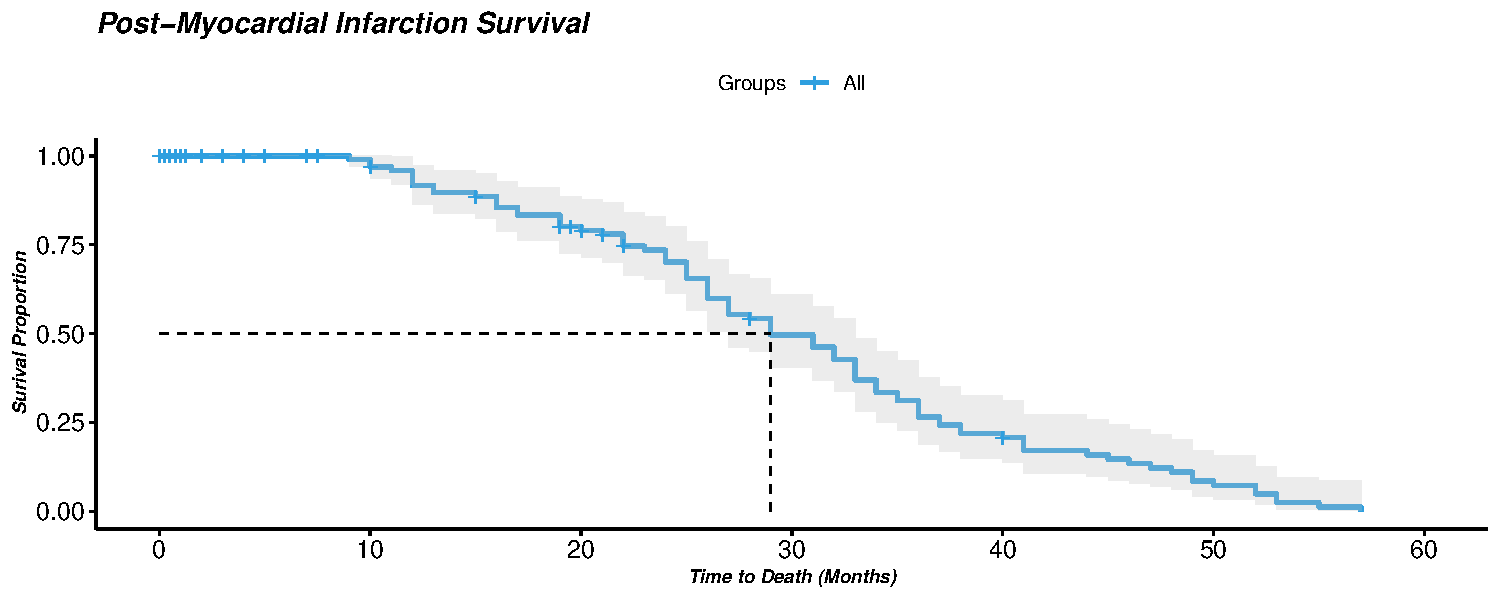
\includegraphics{markdown_files/figure-latex/km.all-1} \end{center}

Here is the survival curve for all groups within our dataset. We see
that a majority of our censored values have very short survival times.
This is very intuitive given to our limited interval study time of a
single year. We clearly see a median survival time of approximately 29
weeks.

\begin{tabular}{r|r|r|r|r|r|r|r|r}
\hline
records & n.max & n.start & events & *rmean & *se(rmean) & median & 0.95LCL & 0.95UCL\\
\hline
130 & 130 & 130 & 88 & 30.53008 & 1.249886 & 29 & 27 & 33\\
\hline
\end{tabular}

\hypertarget{hazard-plots}{%
\subsubsection{Hazard Plots}\label{hazard-plots}}

\hypertarget{weibull-curve}{%
\subsection{Weibull Curve}\label{weibull-curve}}

\hypertarget{cox-proportional-hazard}{%
\subsection{Cox Proportional Hazard}\label{cox-proportional-hazard}}

\hypertarget{model-diagnostics}{%
\subsection{Model Diagnostics}\label{model-diagnostics}}

\hypertarget{aic-bic-and-confidence-intervals}{%
\subsubsection{AIC, BIC, and Confidence
Intervals}\label{aic-bic-and-confidence-intervals}}

\hypertarget{residual-analysisqq-plot}{%
\subsubsection{Residual Analysis/QQ
Plot}\label{residual-analysisqq-plot}}

\hypertarget{discussion}{%
\section{Discussion}\label{discussion}}

\hypertarget{references}{%
\section{References}\label{references}}

Heron, M. Deaths: Leading causes for 2017 pdf icon{[}PDF -- 3 M{]}.
National Vital Statistics Reports;68(6). Accessed November 19, 2019.

Oba S, Sato MA, Takemasa I, Monden M, Matsubara K, Ishii S. A Bayesian
missing value estimation method for gene expression profile data.
Bioinformatics. 2003;19(16):2088‐2096.
\url{doi:10.1093/bioinformatics/btg287}

Daniel J. Stekhoven, Peter Bühlmann, MissForest---non-parametric missing
value imputation for mixed-type data, Bioinformatics, Volume 28, Issue
1, 1 January 2012, Pages 112--118,

Salzberg, S. (1988). Exemplar-based learning: Theory and implementation
(Technical Report TR-10-88). Harvard University, Center for Research in
Computing Technology, Aiken Computation Laboratory (33 Oxford Street;
Cambridge, MA 02138).

Kan, G., Visser, C., Kooler, J., \& Dunning, A. (1986). Short and long
term predictive value of wall motion score in acute myocardial
infarction. British Heart Journal, 56, 422-427.

Fryar CD, Chen T-C, Li X. Prevalence of uncontrolled risk factors for
cardiovascular disease: United States, 1999--2010 pdf
icon{[}PDF-494K{]}. NCHS data brief, no. 103. Hyattsville, MD: National
Center for Health Statistics; 2012. Accessed May 9, 2019.

\hypertarget{appendix}{%
\section{Appendix}\label{appendix}}

\hypertarget{dataset-variable-summary}{%
\subsection{Dataset Variable Summary}\label{dataset-variable-summary}}

\begin{tabu} to \linewidth {>{\raggedright}X>{\raggedright}X>{\raggedright}X}
\hline
Variable & Label & Definition\\
\hline
Survival & Survival & The number of months the patints survived, post-myocardial infarction.\\
\hline
Status & Status & Censorship status. 0 denotes that a patient is a censored while 1 denotes that a patient is uncensored.\\
\hline
Alive at the end of Survival Period & Alive.E & Binary variable. 0 denotes that patient is alive at the end of the survival period while 1 indicates that a patient is still alive.\\
\hline
Patient Age & Age & The age in years when a myocardial infarction occurs.\\
\hline
Age Group & Age.Strata & 0 denotes 49 or younger. 1 denotes 50 or older. 2 denotes 65 or older.\\
\hline
Pericardial Effusion & P.Effusion & Binary variable. Pericardial effusion is excess fluid surrounding the heart. Though excess is not harmful, it is sometimes indicates a porly functioning heart. 0 denotes that pericardial effusion is absent while 1 denotes that fluid is present.\\
\hline
Fractional Shortening & F.Shortening & Fractional shortening is a measure of contractility around the heart. Generally, lower numbers are considered to be abnormal.\\
\hline
E-Point Septal Separation & EPSS & E-point septal separation is an addition measure of heart contractivity. Larger numbers are considered to be abnormal.\\
\hline
Left Ventricular End-Diastolic Dimension & LVDD & Left ventricular end-diastolic dimension is the measure of the heart at the end of disatole. The larger this value is indicates a larger heart. Larger hearts are generally in poor health.\\
\hline
Wall Motion Score & WMS & Wall motion score is a measure of how the segments of the left ventricle are moving during systol.\\
\hline
Wall Motion Index & WMI & Wall motion index is the wall motion score divided by the number of segments that are moving. Normally, 12-13 segments can be seen in an echocardiogram.\\
\hline
Wall Motion Strata & WMI.S & Binary Variable. 0 denotes that WMI is less than or equal to 1.28. 1 denotes that WMI is greater than or equal to 1.28.\\
\hline
\end{tabu}

\hypertarget{original-dataset}{%
\subsection{Original Dataset}\label{original-dataset}}

\begin{table}

\caption{\label{tab:Dataset.actual}Dataset}
\centering
\begin{tabular}[t]{r|r|r|r|r|r|r|r|r|r|r|r}
\hline
Survival & Status & Alive.E & Age & Age.Strata & P.Effusion & F.Shortening & EPSS & LVDD & WMS & WMI & WMI.S\\
\hline
11.00 & 1 & 0 & 71.00 & 2 & 0 & 0.260 & 9.000 & 4.600 & 14.00 & 1.000 & 0\\
\hline
19.00 & 1 & 0 & 72.00 & 2 & 0 & 0.380 & 6.000 & 4.100 & 14.00 & 1.700 & 1\\
\hline
16.00 & 1 & 0 & 55.00 & 1 & 0 & 0.260 & 4.000 & 3.420 & 14.00 & 1.000 & 0\\
\hline
57.00 & 1 & 0 & 60.00 & 1 & 0 & 0.253 & 12.062 & 4.603 & 16.00 & 1.450 & 1\\
\hline
19.00 & 0 & 1 & 57.00 & 1 & 0 & 0.160 & 22.000 & 5.750 & 18.00 & 2.250 & 1\\
\hline
26.00 & 1 & 0 & 68.00 & 2 & 0 & 0.260 & 5.000 & 4.310 & 12.00 & 1.000 & 0\\
\hline
13.00 & 1 & 0 & 62.00 & 1 & 0 & 0.230 & 31.000 & 5.430 & 22.50 & 1.875 & 1\\
\hline
50.00 & 1 & 0 & 60.00 & 1 & 0 & 0.330 & 8.000 & 5.250 & 14.00 & 1.000 & 0\\
\hline
19.00 & 1 & 0 & 46.00 & 0 & 0 & 0.340 & 0.000 & 5.090 & 16.00 & 1.140 & 0\\
\hline
25.00 & 1 & 0 & 54.00 & 1 & 0 & 0.140 & 13.000 & 4.490 & 15.50 & 1.190 & 0\\
\hline
10.00 & 0 & 1 & 77.00 & 2 & 0 & 0.130 & 16.000 & 4.230 & 18.00 & 1.800 & 1\\
\hline
52.00 & 1 & 0 & 62.00 & 1 & 1 & 0.450 & 9.000 & 3.600 & 16.00 & 1.140 & 0\\
\hline
52.00 & 1 & 0 & 73.00 & 2 & 0 & 0.330 & 6.000 & 4.000 & 14.00 & 1.000 & 0\\
\hline
44.00 & 1 & 0 & 60.00 & 1 & 0 & 0.150 & 10.000 & 3.730 & 14.00 & 1.000 & 0\\
\hline
0.50 & 0 & 1 & 62.00 & 1 & 0 & 0.120 & 23.000 & 5.800 & 11.67 & 2.330 & 1\\
\hline
24.00 & 1 & 0 & 55.00 & 1 & 1 & 0.250 & 12.063 & 4.290 & 14.00 & 1.000 & 0\\
\hline
0.50 & 0 & 1 & 69.00 & 2 & 1 & 0.260 & 11.000 & 4.650 & 18.00 & 1.640 & 1\\
\hline
0.50 & 0 & 1 & 62.53 & 1 & 1 & 0.070 & 20.000 & 5.200 & 24.00 & 2.000 & 1\\
\hline
22.00 & 0 & 1 & 66.00 & 2 & 0 & 0.090 & 17.000 & 5.819 & 8.00 & 1.333 & 1\\
\hline
1.00 & 0 & 1 & 66.00 & 2 & 1 & 0.220 & 15.000 & 5.400 & 27.00 & 2.250 & 1\\
\hline
0.75 & 0 & 1 & 69.00 & 2 & 0 & 0.150 & 12.000 & 5.390 & 19.50 & 1.625 & 1\\
\hline
0.75 & 0 & 1 & 85.00 & 2 & 1 & 0.180 & 19.000 & 5.460 & 13.83 & 1.380 & 1\\
\hline
0.50 & 0 & 1 & 73.00 & 2 & 0 & 0.230 & 12.733 & 6.060 & 7.50 & 1.500 & 1\\
\hline
5.00 & 0 & 1 & 71.00 & 2 & 0 & 0.170 & 0.000 & 4.650 & 8.00 & 1.000 & 0\\
\hline
48.00 & 1 & 0 & 64.00 & 1 & 0 & 0.190 & 5.900 & 3.480 & 10.00 & 1.110 & 0\\
\hline
29.00 & 1 & 0 & 54.00 & 1 & 0 & 0.300 & 7.000 & 3.850 & 10.00 & 1.667 & 1\\
\hline
29.00 & 1 & 0 & 35.00 & 0 & 0 & 0.300 & 5.000 & 4.170 & 14.00 & 1.000 & 0\\
\hline
29.00 & 1 & 0 & 55.00 & 1 & 0 & NA & 7.000 & NA & 2.00 & 1.000 & 0\\
\hline
0.25 & 0 & 1 & 75.00 & 2 & 0 & NA & NA & NA & NA & 1.000 & 0\\
\hline
36.00 & 1 & 0 & 55.00 & 1 & 1 & 0.210 & 4.200 & 4.160 & 14.00 & 1.560 & 1\\
\hline
1.00 & 0 & 1 & 65.00 & 2 & 0 & 0.150 & NA & 5.050 & 10.00 & 1.000 & 0\\
\hline
1.00 & 0 & 1 & 52.00 & 1 & 1 & 0.170 & 17.200 & 5.320 & 14.00 & 1.170 & 0\\
\hline
3.00 & 0 & 1 & NA & 2 & 0 & NA & 12.000 & NA & 6.00 & 3.000 & 1\\
\hline
27.00 & 1 & 0 & 47.00 & 0 & 0 & 0.400 & 5.120 & 3.100 & 12.00 & 1.000 & 0\\
\hline
35.00 & 1 & 0 & 63.00 & 1 & 0 & NA & 10.000 & NA & 14.00 & 1.170 & 0\\
\hline
26.00 & 1 & 0 & 61.00 & 1 & 0 & 0.610 & 13.100 & 4.070 & 13.00 & 1.625 & 1\\
\hline
16.00 & 1 & 0 & 63.00 & 1 & 1 & NA & NA & 5.310 & 5.00 & 1.000 & 0\\
\hline
1.00 & 0 & 1 & 65.00 & 2 & 0 & 0.060 & 23.600 & NA & 21.50 & 2.150 & 1\\
\hline
19.00 & 1 & 0 & 68.00 & 2 & 0 & 0.510 & NA & 3.880 & 15.00 & 1.670 & 1\\
\hline
31.00 & 1 & 0 & 80.00 & 2 & 0 & 0.410 & 5.400 & 4.360 & NA & 1.000 & 0\\
\hline
32.00 & 1 & 0 & 54.00 & 1 & 0 & 0.350 & 9.300 & 3.630 & 11.00 & 1.222 & 0\\
\hline
16.00 & 1 & 0 & 70.00 & 2 & 1 & 0.270 & 4.700 & 4.490 & 22.00 & 2.000 & 1\\
\hline
40.00 & 1 & 0 & 79.00 & 2 & 0 & 0.150 & 17.500 & 4.270 & 13.00 & 1.300 & 1\\
\hline
46.00 & 1 & 0 & 56.00 & 1 & 0 & 0.330 & NA & 3.590 & 14.00 & 1.000 & 0\\
\hline
2.00 & 0 & 1 & 67.00 & 2 & 1 & 0.440 & 9.000 & 3.960 & 17.50 & 1.450 & 1\\
\hline
37.00 & 1 & 0 & 64.00 & 1 & 0 & 0.090 & NA & NA & 12.00 & 2.000 & 1\\
\hline
19.50 & 0 & 1 & 81.00 & 2 & 0 & 0.120 & NA & NA & 9.00 & 1.250 & 0\\
\hline
20.00 & 0 & 1 & 59.00 & 1 & 0 & 0.030 & 21.300 & 6.290 & 17.00 & 1.310 & 1\\
\hline
0.25 & 0 & 1 & 63.00 & 1 & 1 & NA & NA & NA & 23.00 & 2.300 & 1\\
\hline
2.00 & 0 & 1 & 56.00 & 1 & 1 & 0.040 & 14.000 & 5.000 & NA & NA & 1\\
\hline
7.00 & 0 & 1 & 61.00 & 1 & 1 & 0.270 & NA & NA & 9.00 & 1.500 & 1\\
\hline
10.00 & 1 & 0 & 57.00 & 1 & 0 & 0.240 & 14.800 & 5.260 & 18.00 & 1.380 & 1\\
\hline
12.00 & 1 & 0 & 58.00 & 1 & 0 & 0.300 & 9.400 & 3.490 & 14.00 & 1.000 & 0\\
\hline
1.00 & 0 & 1 & 60.00 & 1 & 0 & 0.010 & 24.600 & 5.650 & 39.00 & 3.000 & 1\\
\hline
10.00 & 1 & 0 & 66.00 & 2 & 0 & 0.290 & 15.600 & 6.150 & 14.00 & 1.000 & 0\\
\hline
45.00 & 1 & 0 & 63.00 & 1 & 0 & 0.150 & 13.000 & 4.570 & 13.00 & 1.080 & 0\\
\hline
22.00 & 1 & 0 & 57.00 & 1 & 0 & 0.130 & 18.600 & 4.370 & 12.33 & 1.370 & 1\\
\hline
53.00 & 1 & 0 & 70.00 & 2 & 0 & 0.100 & 9.800 & 5.300 & 23.00 & 2.300 & 1\\
\hline
38.00 & 1 & 0 & 68.00 & 2 & 0 & 0.290 & NA & 4.410 & 14.00 & 1.167 & 0\\
\hline
26.00 & 1 & 0 & 79.00 & 2 & 0 & 0.170 & 11.900 & 5.150 & 10.50 & 1.050 & 0\\
\hline
9.00 & 1 & 0 & 73.00 & 2 & 0 & 0.120 & NA & 6.780 & 16.67 & 1.390 & 1\\
\hline
26.00 & 1 & 0 & 72.00 & 2 & 0 & 0.187 & 12.000 & 5.020 & 13.00 & 1.180 & 0\\
\hline
0.50 & 0 & 1 & 59.00 & 1 & 0 & 0.130 & 16.400 & 4.960 & 17.83 & 1.370 & 1\\
\hline
12.00 & 1 & 0 & 67.00 & 2 & 1 & 0.110 & 10.300 & 4.680 & 11.00 & 1.000 & 0\\
\hline
49.00 & 1 & 0 & 51.00 & 1 & 0 & 0.160 & 13.200 & 5.260 & 11.00 & 1.000 & 0\\
\hline
0.75 & 0 & 1 & 50.00 & 1 & 0 & 0.140 & 11.400 & 4.750 & 10.00 & 2.500 & 1\\
\hline
49.00 & 1 & 0 & 70.00 & 2 & 1 & 0.250 & 9.700 & 5.570 & 5.50 & 1.100 & 0\\
\hline
47.00 & 1 & 0 & 65.00 & 2 & 0 & 0.360 & 8.800 & 5.780 & 12.00 & 1.000 & 0\\
\hline
41.00 & 1 & 0 & 78.00 & 2 & 0 & 0.060 & 16.100 & 5.620 & 13.67 & 1.367 & 1\\
\hline
0.25 & 0 & 1 & 86.00 & 2 & 0 & 0.225 & 12.200 & 5.200 & 24.00 & 2.180 & 1\\
\hline
33.00 & 1 & 0 & 56.00 & 1 & 0 & 0.250 & 11.000 & 4.720 & 11.00 & 1.000 & 0\\
\hline
29.00 & 1 & 0 & 60.00 & 1 & 0 & 0.120 & 10.200 & 4.310 & 15.00 & 1.670 & 1\\
\hline
41.00 & 1 & 0 & 59.00 & 1 & 0 & 0.290 & 7.500 & 4.750 & 13.00 & 1.080 & 0\\
\hline
26.00 & 1 & 0 & 50.00 & 1 & 0 & 0.060 & 30.100 & 5.950 & 21.50 & 2.390 & 1\\
\hline
15.00 & 1 & 0 & 54.00 & 1 & 0 & 0.217 & 17.900 & 4.540 & 16.50 & 1.180 & 0\\
\hline
0.25 & 0 & 1 & 68.00 & 2 & 0 & 0.220 & 21.700 & 4.850 & 15.00 & 1.150 & 0\\
\hline
0.03 & 0 & 1 & NA & 2 & 0 & 0.260 & 19.400 & 4.770 & 21.00 & 2.100 & 1\\
\hline
12.00 & 1 & 0 & 64.00 & 1 & 0 & 0.200 & 7.100 & 4.580 & 14.00 & 1.000 & 0\\
\hline
32.00 & 1 & 0 & 63.00 & 1 & 0 & 0.200 & 5.000 & 5.200 & 8.00 & 1.000 & 0\\
\hline
32.00 & 1 & 0 & 65.00 & 2 & 0 & 0.060 & 23.600 & 6.740 & 12.00 & 1.090 & 0\\
\hline
27.00 & 1 & 0 & 54.00 & 1 & 1 & 0.070 & 16.800 & 4.160 & 18.00 & 1.500 & 1\\
\hline
23.00 & 1 & 0 & 62.00 & 1 & 0 & 0.250 & 6.000 & 4.480 & 11.00 & 1.000 & 0\\
\hline
0.75 & 0 & 1 & 78.00 & 2 & 0 & 0.050 & 10.000 & 4.440 & 15.00 & 1.360 & 1\\
\hline
0.75 & 0 & 1 & 61.00 & 1 & 0 & NA & NA & NA & 28.00 & 2.330 & 1\\
\hline
34.00 & 1 & 0 & 52.00 & 1 & 0 & 0.140 & 25.000 & 6.210 & 11.50 & 1.150 & 0\\
\hline
1.00 & 0 & 1 & 73.00 & 2 & 0 & 0.050 & 14.800 & 4.140 & 15.50 & 1.410 & 1\\
\hline
21.00 & 0 & 1 & 70.00 & 2 & 1 & 0.160 & 19.200 & 5.250 & 11.00 & 1.000 & 0\\
\hline
55.00 & 1 & 0 & 55.00 & 1 & 0 & 0.280 & 5.500 & 4.480 & 22.00 & 1.830 & 1\\
\hline
15.00 & 0 & 1 & 60.00 & 1 & 0 & 0.180 & 8.700 & 4.560 & 13.50 & 1.040 & 0\\
\hline
0.50 & 0 & 1 & 67.00 & 2 & 0 & 0.155 & 11.300 & 5.160 & 13.00 & 1.000 & 0\\
\hline
35.00 & 1 & 0 & 64.00 & 1 & 0 & 0.300 & 6.600 & 4.360 & 14.00 & 1.270 & 0\\
\hline
53.00 & 1 & 0 & 59.00 & 1 & 0 & 0.344 & 9.100 & 4.040 & 9.00 & 1.000 & 0\\
\hline
33.00 & 1 & 0 & 46.00 & 0 & 0 & 0.272 & 16.500 & 5.360 & 12.67 & 1.060 & 0\\
\hline
33.00 & 1 & 0 & 63.00 & 1 & 0 & 0.250 & 5.600 & 3.870 & 18.00 & 1.500 & 1\\
\hline
40.00 & 0 & 1 & 74.00 & 2 & 0 & 0.200 & 4.800 & 4.560 & 12.50 & 1.040 & 0\\
\hline
33.00 & 1 & 0 & 59.00 & 1 & 0 & 0.500 & 9.100 & 3.420 & 18.00 & 1.500 & 1\\
\hline
5.00 & 0 & 1 & 65.00 & 2 & 1 & 0.160 & 8.500 & 5.470 & 16.00 & 1.450 & 1\\
\hline
4.00 & 0 & 1 & 58.00 & 1 & 0 & 0.170 & 28.900 & 6.730 & 26.08 & 2.010 & 1\\
\hline
31.00 & 1 & 0 & 53.00 & 1 & 0 & 0.170 & NA & 4.690 & 10.00 & 1.000 & 0\\
\hline
33.00 & 1 & 0 & 66.00 & 2 & 0 & 0.200 & NA & 4.230 & 12.00 & 1.000 & 0\\
\hline
22.00 & 1 & 0 & 70.00 & 2 & 0 & 0.380 & 0.000 & 4.550 & 10.00 & 1.000 & 0\\
\hline
25.00 & 1 & 0 & 62.00 & 1 & 0 & 0.258 & 11.800 & 4.870 & 11.00 & 1.000 & 0\\
\hline
1.25 & 0 & 1 & 63.00 & 1 & 0 & 0.300 & 6.900 & 3.520 & 18.16 & 1.510 & 1\\
\hline
24.00 & 1 & 0 & 59.00 & 1 & 0 & 0.170 & 14.300 & 5.490 & 13.50 & 1.500 & 1\\
\hline
25.00 & 1 & 0 & 57.00 & 1 & 0 & 0.228 & 9.700 & 4.290 & 11.00 & 1.000 & 0\\
\hline
24.00 & 1 & 0 & 57.00 & 1 & 0 & 0.036 & 7.000 & 4.120 & 13.50 & 1.230 & 0\\
\hline
0.75 & 0 & 1 & 78.00 & 2 & 0 & 0.230 & 40.000 & 6.230 & 14.00 & 1.400 & 1\\
\hline
3.00 & 0 & 1 & 62.00 & 1 & 0 & 0.260 & 7.600 & 4.420 & 14.00 & 1.000 & 0\\
\hline
27.00 & 1 & 0 & 62.00 & 1 & 0 & 0.220 & 12.100 & 3.920 & 11.00 & 1.000 & 0\\
\hline
13.00 & 1 & 0 & 66.00 & 2 & 0 & 0.240 & 13.600 & 4.380 & 22.00 & 2.200 & 1\\
\hline
36.00 & 1 & 0 & 61.00 & 1 & 0 & 0.270 & 9.000 & 4.060 & 12.00 & 1.000 & 0\\
\hline
25.00 & 1 & 0 & 59.00 & 1 & 1 & 0.400 & 9.200 & 5.360 & 12.00 & 1.000 & 0\\
\hline
27.00 & 1 & 0 & 57.00 & 1 & 0 & 0.290 & 9.400 & 4.770 & 9.00 & 1.000 & 0\\
\hline
34.00 & 1 & 0 & 62.00 & 1 & 1 & 0.190 & 28.900 & 6.630 & 19.50 & 1.950 & 1\\
\hline
37.00 & 1 & 0 & NA & 2 & 0 & 0.260 & 0.000 & 4.380 & 9.00 & 1.000 & 0\\
\hline
34.00 & 1 & 0 & 54.00 & 1 & 0 & 0.430 & 9.300 & 4.790 & 10.00 & 1.000 & 0\\
\hline
28.00 & 0 & 1 & 62.00 & 1 & 1 & 0.240 & 28.600 & 5.860 & 21.50 & 1.950 & 1\\
\hline
28.00 & 1 & 0 & NA & 2 & 0 & 0.230 & 19.100 & 5.490 & 12.00 & 1.200 & 0\\
\hline
17.00 & 1 & 0 & 64.00 & 1 & 0 & 0.150 & 6.600 & 4.170 & 14.00 & 1.270 & 0\\
\hline
38.00 & 1 & 0 & 57.00 & 1 & 1 & 0.120 & 0.000 & 2.320 & 16.50 & 1.375 & 1\\
\hline
31.00 & 1 & 0 & 61.00 & 1 & 0 & 0.180 & 0.000 & 4.480 & 11.00 & 1.375 & 1\\
\hline
12.00 & 1 & 0 & 61.00 & 1 & 1 & 0.190 & 13.200 & 5.040 & 19.00 & 1.730 & 1\\
\hline
36.00 & 1 & 0 & 48.00 & 0 & 0 & 0.150 & 12.000 & 3.660 & 10.00 & 1.000 & 0\\
\hline
17.00 & 1 & 0 & NA & 2 & 0 & 0.090 & 6.800 & 4.960 & 13.00 & 1.080 & 0\\
\hline
21.00 & 1 & 0 & 61.00 & 1 & 0 & 0.140 & 25.500 & 5.160 & 14.00 & 1.270 & 0\\
\hline
7.50 & 0 & 1 & 64.00 & 1 & 0 & 0.240 & 12.900 & 4.720 & 12.00 & 1.000 & 0\\
\hline
41.00 & 1 & 0 & 64.00 & 1 & 0 & 0.280 & 5.400 & 5.470 & 11.00 & 1.100 & 0\\
\hline
36.00 & 1 & 0 & 69.00 & 2 & 0 & 0.200 & 7.000 & 5.050 & 14.50 & 1.210 & 0\\
\hline
22.00 & 1 & 0 & 57.00 & 1 & 0 & 0.140 & 16.100 & 4.360 & 15.00 & 1.360 & 1\\
\hline
20.00 & 1 & 0 & 62.00 & 1 & 0 & 0.150 & 0.000 & 4.510 & 15.50 & 1.409 & 1\\
\hline
\end{tabular}
\end{table}

\hypertarget{imputed-dataset}{%
\subsection{Imputed Dataset}\label{imputed-dataset}}

missForest iteration 1 in progress\ldots{}

\begin{verbatim}
## Warning in randomForest.default(x = obsX, y = obsY, ntree = ntree, mtry =
## mtry, : The response has five or fewer unique values. Are you sure you want to
## do regression?

## Warning in randomForest.default(x = obsX, y = obsY, ntree = ntree, mtry =
## mtry, : The response has five or fewer unique values. Are you sure you want to
## do regression?

## Warning in randomForest.default(x = obsX, y = obsY, ntree = ntree, mtry =
## mtry, : The response has five or fewer unique values. Are you sure you want to
## do regression?

## Warning in randomForest.default(x = obsX, y = obsY, ntree = ntree, mtry =
## mtry, : The response has five or fewer unique values. Are you sure you want to
## do regression?

## Warning in randomForest.default(x = obsX, y = obsY, ntree = ntree, mtry =
## mtry, : The response has five or fewer unique values. Are you sure you want to
## do regression?
\end{verbatim}

done! missForest iteration 2 in progress\ldots{}

\begin{verbatim}
## Warning in randomForest.default(x = obsX, y = obsY, ntree = ntree, mtry =
## mtry, : The response has five or fewer unique values. Are you sure you want to
## do regression?

## Warning in randomForest.default(x = obsX, y = obsY, ntree = ntree, mtry =
## mtry, : The response has five or fewer unique values. Are you sure you want to
## do regression?

## Warning in randomForest.default(x = obsX, y = obsY, ntree = ntree, mtry =
## mtry, : The response has five or fewer unique values. Are you sure you want to
## do regression?

## Warning in randomForest.default(x = obsX, y = obsY, ntree = ntree, mtry =
## mtry, : The response has five or fewer unique values. Are you sure you want to
## do regression?

## Warning in randomForest.default(x = obsX, y = obsY, ntree = ntree, mtry =
## mtry, : The response has five or fewer unique values. Are you sure you want to
## do regression?
\end{verbatim}

done! missForest iteration 3 in progress\ldots{}

\begin{verbatim}
## Warning in randomForest.default(x = obsX, y = obsY, ntree = ntree, mtry =
## mtry, : The response has five or fewer unique values. Are you sure you want to
## do regression?

## Warning in randomForest.default(x = obsX, y = obsY, ntree = ntree, mtry =
## mtry, : The response has five or fewer unique values. Are you sure you want to
## do regression?

## Warning in randomForest.default(x = obsX, y = obsY, ntree = ntree, mtry =
## mtry, : The response has five or fewer unique values. Are you sure you want to
## do regression?

## Warning in randomForest.default(x = obsX, y = obsY, ntree = ntree, mtry =
## mtry, : The response has five or fewer unique values. Are you sure you want to
## do regression?

## Warning in randomForest.default(x = obsX, y = obsY, ntree = ntree, mtry =
## mtry, : The response has five or fewer unique values. Are you sure you want to
## do regression?
\end{verbatim}

done! missForest iteration 4 in progress\ldots{}

\begin{verbatim}
## Warning in randomForest.default(x = obsX, y = obsY, ntree = ntree, mtry =
## mtry, : The response has five or fewer unique values. Are you sure you want to
## do regression?

## Warning in randomForest.default(x = obsX, y = obsY, ntree = ntree, mtry =
## mtry, : The response has five or fewer unique values. Are you sure you want to
## do regression?

## Warning in randomForest.default(x = obsX, y = obsY, ntree = ntree, mtry =
## mtry, : The response has five or fewer unique values. Are you sure you want to
## do regression?

## Warning in randomForest.default(x = obsX, y = obsY, ntree = ntree, mtry =
## mtry, : The response has five or fewer unique values. Are you sure you want to
## do regression?

## Warning in randomForest.default(x = obsX, y = obsY, ntree = ntree, mtry =
## mtry, : The response has five or fewer unique values. Are you sure you want to
## do regression?
\end{verbatim}

done! missForest iteration 5 in progress\ldots{}

\begin{verbatim}
## Warning in randomForest.default(x = obsX, y = obsY, ntree = ntree, mtry =
## mtry, : The response has five or fewer unique values. Are you sure you want to
## do regression?

## Warning in randomForest.default(x = obsX, y = obsY, ntree = ntree, mtry =
## mtry, : The response has five or fewer unique values. Are you sure you want to
## do regression?

## Warning in randomForest.default(x = obsX, y = obsY, ntree = ntree, mtry =
## mtry, : The response has five or fewer unique values. Are you sure you want to
## do regression?

## Warning in randomForest.default(x = obsX, y = obsY, ntree = ntree, mtry =
## mtry, : The response has five or fewer unique values. Are you sure you want to
## do regression?

## Warning in randomForest.default(x = obsX, y = obsY, ntree = ntree, mtry =
## mtry, : The response has five or fewer unique values. Are you sure you want to
## do regression?
\end{verbatim}

done!

\begin{tabular}{r|r|r|r|r|r|r|r|r|r|r|r}
\hline
Survival & Status & Alive.E & Age & Age.Strata & P.Effusion & F.Shortening & EPSS & LVDD & WMS & WMI & WMI.S\\
\hline
11.00 & 1.00 & 0.00 & 71.00 & 2.00 & 0.00 & 0.26 & 9.00 & 4.60 & 14.00 & 1.08 & 0.00\\
\hline
19.00 & 0.97 & 0.00 & 72.00 & 1.84 & 0.00 & 0.38 & 6.00 & 4.10 & 14.00 & 1.70 & 1.00\\
\hline
16.00 & 0.98 & 0.00 & 55.00 & 1.00 & 0.00 & 0.26 & 4.00 & 3.42 & 14.00 & 1.00 & 0.00\\
\hline
57.00 & 1.00 & 0.00 & 60.00 & 1.00 & 0.00 & 0.25 & 12.06 & 4.60 & 16.00 & 1.45 & 1.00\\
\hline
19.00 & 0.28 & 0.68 & 60.15 & 1.00 & 0.00 & 0.16 & 22.00 & 5.75 & 18.00 & 1.57 & 1.00\\
\hline
26.00 & 1.00 & 0.00 & 68.00 & 2.00 & 0.00 & 0.26 & 7.30 & 4.31 & 12.00 & 1.00 & 0.00\\
\hline
13.00 & 1.00 & 0.00 & 62.00 & 1.00 & 0.00 & 0.23 & 31.00 & 5.43 & 22.50 & 1.88 & 1.00\\
\hline
50.00 & 1.00 & 0.01 & 60.00 & 1.00 & 0.00 & 0.33 & 8.00 & 5.25 & 14.00 & 1.00 & 0.00\\
\hline
19.00 & 1.00 & 0.00 & 46.00 & 0.00 & 0.00 & 0.25 & 0.00 & 5.09 & 16.00 & 1.14 & 0.00\\
\hline
25.00 & 1.00 & 0.00 & 54.00 & 1.00 & 0.00 & 0.14 & 13.00 & 4.49 & 15.50 & 1.19 & 0.00\\
\hline
10.00 & 0.00 & 1.00 & 77.00 & 2.00 & 0.00 & 0.13 & 16.00 & 4.23 & 18.00 & 1.80 & 1.00\\
\hline
52.00 & 1.00 & 0.00 & 58.12 & 1.00 & 1.00 & 0.45 & 9.00 & 3.60 & 16.00 & 1.14 & 0.00\\
\hline
52.00 & 0.95 & 0.00 & 73.00 & 2.00 & 0.00 & 0.33 & 6.00 & 4.00 & 14.00 & 1.00 & 0.00\\
\hline
31.78 & 1.00 & 0.00 & 60.00 & 1.00 & 0.00 & 0.15 & 10.00 & 3.73 & 14.00 & 1.00 & 0.00\\
\hline
0.50 & 0.00 & 1.00 & 62.00 & 1.00 & 0.00 & 0.12 & 23.00 & 5.80 & 11.67 & 2.33 & 1.00\\
\hline
24.00 & 1.00 & 0.00 & 55.00 & 1.00 & 1.00 & 0.25 & 12.06 & 4.66 & 9.36 & 1.00 & 0.00\\
\hline
0.50 & 0.00 & 1.00 & 69.00 & 2.00 & 1.00 & 0.26 & 11.00 & 4.65 & 14.73 & 1.64 & 1.00\\
\hline
0.50 & 0.00 & 1.00 & 62.53 & 1.00 & 1.00 & 0.19 & 19.83 & 5.45 & 24.00 & 2.00 & 1.00\\
\hline
22.00 & 0.00 & 0.71 & 66.00 & 2.00 & 0.00 & 0.09 & 19.03 & 5.82 & 8.00 & 1.33 & 1.00\\
\hline
1.00 & 0.01 & 1.00 & 66.00 & 2.00 & 1.00 & 0.22 & 15.00 & 5.40 & 27.00 & 2.25 & 1.00\\
\hline
0.75 & 0.00 & 1.00 & 69.00 & 2.00 & 0.00 & 0.15 & 12.00 & 5.39 & 19.50 & 1.62 & 1.00\\
\hline
0.75 & 0.00 & 1.00 & 85.00 & 2.00 & 1.00 & 0.18 & 19.00 & 5.46 & 13.83 & 1.38 & 1.00\\
\hline
0.50 & 0.00 & 1.00 & 73.00 & 2.00 & 0.00 & 0.23 & 12.73 & 6.06 & 7.50 & 1.50 & 1.00\\
\hline
5.00 & 0.16 & 1.00 & 71.00 & 1.82 & 0.00 & 0.25 & 0.00 & 4.65 & 8.00 & 1.00 & 0.00\\
\hline
48.00 & 1.00 & 0.00 & 64.00 & 1.00 & 0.00 & 0.19 & 9.07 & 3.48 & 10.00 & 1.11 & 0.00\\
\hline
29.00 & 1.00 & 0.00 & 54.00 & 1.00 & 0.00 & 0.30 & 7.00 & 3.85 & 10.00 & 1.67 & 1.00\\
\hline
29.00 & 1.00 & 0.00 & 35.00 & 0.64 & 0.00 & 0.30 & 5.00 & 4.17 & 14.00 & 1.00 & 0.00\\
\hline
29.00 & 1.00 & 0.00 & 55.00 & 1.00 & 0.00 & 0.28 & 7.00 & 4.35 & 2.00 & 1.00 & 0.00\\
\hline
0.25 & 0.00 & 1.00 & 75.00 & 2.00 & 0.10 & 0.21 & 14.64 & 5.01 & 14.31 & 1.20 & 0.00\\
\hline
36.00 & 1.00 & 0.00 & 55.00 & 1.00 & 1.00 & 0.21 & 4.20 & 4.16 & 14.00 & 1.56 & 1.00\\
\hline
1.00 & 0.00 & 0.96 & 65.00 & 2.00 & 0.00 & 0.15 & 12.38 & 5.05 & 10.00 & 1.00 & 0.00\\
\hline
1.00 & 0.03 & 1.00 & 52.00 & 1.14 & 1.00 & 0.18 & 17.20 & 5.32 & 14.90 & 1.17 & 0.00\\
\hline
3.00 & 0.00 & 1.00 & 68.49 & 2.00 & 0.00 & 0.14 & 12.00 & 5.23 & 6.00 & 3.00 & 1.00\\
\hline
27.00 & 1.00 & 0.00 & 47.00 & 0.00 & 0.00 & 0.40 & 5.12 & 3.10 & 12.00 & 1.00 & 0.00\\
\hline
35.00 & 1.00 & 0.00 & 63.00 & 1.00 & 0.00 & 0.18 & 10.00 & 4.34 & 14.00 & 1.17 & 0.00\\
\hline
26.00 & 1.00 & 0.00 & 61.00 & 1.00 & 0.00 & 0.61 & 13.10 & 4.07 & 15.28 & 1.62 & 1.00\\
\hline
30.87 & 1.00 & 0.00 & 63.00 & 1.09 & 1.00 & 0.28 & 8.47 & 4.81 & 5.00 & 1.07 & 0.00\\
\hline
1.00 & 0.00 & 1.00 & 70.18 & 2.00 & 0.00 & 0.06 & 15.48 & 5.17 & 21.50 & 2.15 & 1.00\\
\hline
19.00 & 1.00 & 0.00 & 68.00 & 2.00 & 0.00 & 0.51 & 8.55 & 3.88 & 15.00 & 1.67 & 1.00\\
\hline
31.00 & 1.00 & 0.00 & 80.00 & 2.00 & 0.20 & 0.41 & 5.40 & 4.36 & 10.84 & 1.00 & 0.00\\
\hline
29.98 & 1.00 & 0.00 & 54.00 & 1.00 & 0.04 & 0.27 & 9.30 & 3.63 & 11.00 & 1.22 & 0.00\\
\hline
16.00 & 1.00 & 0.00 & 70.00 & 2.00 & 1.00 & 0.27 & 4.70 & 4.49 & 18.75 & 2.00 & 0.92\\
\hline
40.00 & 1.00 & 0.00 & 79.00 & 2.00 & 0.00 & 0.15 & 17.50 & 4.27 & 13.00 & 1.30 & 1.00\\
\hline
46.00 & 1.00 & 0.01 & 56.00 & 1.00 & 0.00 & 0.33 & 8.20 & 3.59 & 14.00 & 1.00 & 0.00\\
\hline
2.00 & 0.00 & 1.00 & 67.00 & 2.00 & 1.00 & 0.44 & 9.00 & 3.96 & 17.50 & 1.45 & 1.00\\
\hline
37.00 & 1.00 & 0.00 & 64.00 & 1.00 & 0.00 & 0.09 & 9.85 & 4.41 & 12.00 & 1.41 & 1.00\\
\hline
19.50 & 0.00 & 1.00 & 81.00 & 2.00 & 0.00 & 0.12 & 12.69 & 4.84 & 9.00 & 1.25 & 0.00\\
\hline
20.00 & 0.00 & 0.65 & 59.00 & 1.00 & 0.00 & 0.03 & 21.30 & 6.29 & 17.00 & 1.31 & 1.00\\
\hline
0.25 & 0.00 & 1.00 & 63.00 & 1.00 & 1.00 & 0.18 & 16.87 & 5.30 & 23.00 & 2.30 & 1.00\\
\hline
2.00 & 0.00 & 1.00 & 56.00 & 1.00 & 1.00 & 0.04 & 14.00 & 5.00 & 21.18 & 1.88 & 1.00\\
\hline
7.00 & 0.00 & 1.00 & 61.00 & 1.20 & 1.00 & 0.27 & 10.07 & 4.83 & 9.00 & 1.50 & 1.00\\
\hline
10.00 & 1.00 & 0.00 & 59.71 & 1.00 & 0.00 & 0.24 & 14.80 & 5.26 & 18.00 & 1.38 & 1.00\\
\hline
12.00 & 1.00 & 0.00 & 58.00 & 1.00 & 0.00 & 0.30 & 9.40 & 3.49 & 14.00 & 1.00 & 0.00\\
\hline
1.00 & 0.00 & 1.00 & 60.00 & 1.00 & 0.00 & 0.01 & 24.60 & 5.65 & 39.00 & 3.00 & 1.00\\
\hline
10.00 & 1.00 & 0.00 & 66.00 & 2.00 & 0.00 & 0.29 & 14.77 & 6.15 & 14.00 & 1.00 & 0.00\\
\hline
45.00 & 1.00 & 0.00 & 63.00 & 1.00 & 0.00 & 0.15 & 13.00 & 4.57 & 13.00 & 1.08 & 0.00\\
\hline
22.00 & 1.00 & 0.00 & 57.00 & 1.02 & 0.00 & 0.13 & 12.14 & 4.37 & 12.33 & 1.46 & 1.00\\
\hline
53.00 & 1.00 & 0.00 & 70.00 & 2.00 & 0.00 & 0.10 & 9.80 & 5.30 & 23.00 & 1.74 & 1.00\\
\hline
38.00 & 1.00 & 0.00 & 68.00 & 2.00 & 0.00 & 0.29 & 6.61 & 4.41 & 14.00 & 1.17 & 0.00\\
\hline
26.00 & 1.00 & 0.00 & 79.00 & 1.82 & 0.00 & 0.17 & 10.92 & 5.15 & 10.50 & 1.05 & 0.00\\
\hline
9.00 & 1.00 & 0.00 & 68.96 & 2.00 & 0.16 & 0.12 & 19.61 & 6.78 & 16.67 & 1.52 & 1.00\\
\hline
26.00 & 0.94 & 0.00 & 72.00 & 2.00 & 0.00 & 0.19 & 12.00 & 5.02 & 13.00 & 1.18 & 0.00\\
\hline
0.50 & 0.00 & 1.00 & 59.00 & 1.00 & 0.00 & 0.15 & 14.53 & 4.96 & 17.83 & 1.37 & 1.00\\
\hline
12.00 & 1.00 & 0.00 & 67.00 & 2.00 & 1.00 & 0.11 & 10.30 & 4.68 & 11.00 & 1.00 & 0.00\\
\hline
49.00 & 1.00 & 0.00 & 51.00 & 1.00 & 0.00 & 0.16 & 13.20 & 5.26 & 11.00 & 1.00 & 0.00\\
\hline
0.75 & 0.00 & 1.00 & 50.00 & 1.00 & 0.00 & 0.14 & 11.40 & 4.75 & 10.00 & 2.50 & 0.84\\
\hline
49.00 & 1.00 & 0.00 & 70.00 & 2.00 & 1.00 & 0.25 & 9.70 & 5.57 & 5.50 & 1.10 & 0.00\\
\hline
47.00 & 1.00 & 0.00 & 65.00 & 2.00 & 0.00 & 0.36 & 8.80 & 5.78 & 12.00 & 1.00 & 0.00\\
\hline
41.00 & 1.00 & 0.00 & 78.00 & 2.00 & 0.00 & 0.06 & 15.99 & 5.62 & 13.67 & 1.37 & 1.00\\
\hline
0.25 & 0.00 & 1.00 & 60.65 & 1.10 & 0.00 & 0.22 & 12.20 & 5.20 & 24.00 & 2.18 & 1.00\\
\hline
33.00 & 1.00 & 0.00 & 56.00 & 1.00 & 0.00 & 0.25 & 11.00 & 4.72 & 11.00 & 1.00 & 0.00\\
\hline
29.00 & 1.00 & 0.00 & 57.92 & 1.00 & 0.00 & 0.12 & 10.20 & 4.31 & 15.00 & 1.67 & 1.00\\
\hline
41.00 & 1.00 & 0.02 & 59.00 & 1.06 & 0.06 & 0.29 & 7.50 & 4.75 & 13.00 & 1.08 & 0.00\\
\hline
26.00 & 1.00 & 0.00 & 50.00 & 1.00 & 0.00 & 0.06 & 30.10 & 5.95 & 21.50 & 2.39 & 0.91\\
\hline
15.00 & 1.00 & 0.00 & 54.00 & 1.01 & 0.00 & 0.22 & 17.90 & 4.54 & 16.50 & 1.15 & 0.00\\
\hline
0.25 & 0.00 & 1.00 & 68.00 & 1.95 & 0.00 & 0.22 & 13.12 & 4.85 & 15.00 & 1.15 & 0.00\\
\hline
0.03 & 0.00 & 1.00 & 71.17 & 2.00 & 0.00 & 0.26 & 19.40 & 4.77 & 21.00 & 1.89 & 1.00\\
\hline
12.00 & 1.00 & 0.00 & 64.00 & 1.00 & 0.00 & 0.20 & 7.10 & 4.40 & 14.00 & 1.12 & 0.00\\
\hline
32.00 & 1.00 & 0.00 & 63.00 & 1.00 & 0.00 & 0.20 & 5.00 & 5.20 & 8.00 & 1.00 & 0.04\\
\hline
32.00 & 1.00 & 0.00 & 65.00 & 2.00 & 0.00 & 0.06 & 11.71 & 4.94 & 12.00 & 1.09 & 0.00\\
\hline
27.00 & 1.00 & 0.00 & 54.00 & 1.00 & 1.00 & 0.07 & 10.37 & 4.16 & 18.00 & 1.50 & 1.00\\
\hline
23.00 & 1.00 & 0.01 & 62.00 & 1.00 & 0.08 & 0.25 & 6.00 & 4.48 & 11.00 & 1.00 & 0.00\\
\hline
9.43 & 0.00 & 1.00 & 78.00 & 2.00 & 0.00 & 0.05 & 10.00 & 4.44 & 15.00 & 1.36 & 1.00\\
\hline
0.75 & 0.00 & 1.00 & 61.00 & 1.00 & 0.00 & 0.14 & 15.56 & 5.15 & 17.76 & 2.33 & 1.00\\
\hline
29.49 & 1.00 & 0.00 & 52.00 & 1.01 & 0.00 & 0.14 & 25.00 & 6.21 & 11.50 & 1.15 & 0.00\\
\hline
1.00 & 0.00 & 1.00 & 73.00 & 2.00 & 0.23 & 0.05 & 14.80 & 4.14 & 15.50 & 1.41 & 1.00\\
\hline
21.00 & 0.00 & 1.00 & 70.00 & 2.00 & 1.00 & 0.16 & 19.20 & 5.25 & 11.00 & 1.00 & 0.00\\
\hline
25.41 & 1.00 & 0.00 & 55.00 & 1.00 & 0.00 & 0.28 & 5.50 & 4.48 & 22.00 & 1.83 & 1.00\\
\hline
15.00 & 0.40 & 1.00 & 60.00 & 1.00 & 0.00 & 0.18 & 8.70 & 4.56 & 12.86 & 1.04 & 0.00\\
\hline
0.50 & 0.00 & 1.00 & 67.00 & 2.00 & 0.00 & 0.19 & 11.30 & 5.16 & 13.00 & 1.00 & 0.00\\
\hline
35.00 & 1.00 & 0.00 & 64.00 & 1.00 & 0.00 & 0.30 & 6.60 & 4.05 & 14.00 & 1.27 & 0.00\\
\hline
53.00 & 1.00 & 0.00 & 59.00 & 1.00 & 0.00 & 0.34 & 9.10 & 4.04 & 9.00 & 1.00 & 0.00\\
\hline
33.00 & 1.00 & 0.00 & 46.00 & 0.00 & 0.00 & 0.27 & 16.50 & 5.36 & 12.67 & 1.06 & 0.00\\
\hline
33.00 & 0.97 & 0.00 & 63.00 & 1.00 & 0.00 & 0.25 & 5.60 & 3.87 & 18.00 & 1.50 & 1.00\\
\hline
40.00 & 0.00 & 1.00 & 74.00 & 2.00 & 0.00 & 0.20 & 4.80 & 4.56 & 12.50 & 1.04 & 0.00\\
\hline
33.00 & 1.00 & 0.00 & 59.00 & 1.00 & 0.00 & 0.50 & 9.10 & 3.42 & 18.00 & 1.50 & 0.92\\
\hline
5.00 & 0.00 & 1.00 & 65.00 & 2.00 & 1.00 & 0.25 & 8.50 & 5.47 & 16.00 & 1.45 & 1.00\\
\hline
4.00 & 0.00 & 0.89 & 58.00 & 1.00 & 0.00 & 0.17 & 28.90 & 6.73 & 26.08 & 2.01 & 1.00\\
\hline
31.00 & 1.00 & 0.00 & 53.00 & 1.00 & 0.00 & 0.30 & 8.68 & 4.01 & 10.00 & 1.00 & 0.00\\
\hline
33.00 & 1.00 & 0.00 & 66.00 & 1.77 & 0.00 & 0.20 & 8.33 & 4.23 & 12.00 & 1.00 & 0.00\\
\hline
22.00 & 1.00 & 0.04 & 70.00 & 2.00 & 0.21 & 0.38 & 0.00 & 4.55 & 10.00 & 1.00 & 0.00\\
\hline
25.00 & 1.00 & 0.00 & 57.40 & 1.00 & 0.00 & 0.26 & 11.80 & 4.87 & 11.00 & 1.02 & 0.00\\
\hline
1.25 & 0.00 & 1.00 & 63.00 & 1.00 & 0.00 & 0.30 & 6.90 & 3.52 & 18.16 & 1.51 & 0.96\\
\hline
24.00 & 1.00 & 0.00 & 59.00 & 1.00 & 0.00 & 0.19 & 14.30 & 5.49 & 13.50 & 1.50 & 1.00\\
\hline
25.00 & 1.00 & 0.00 & 57.00 & 1.00 & 0.00 & 0.25 & 9.70 & 4.29 & 11.00 & 1.00 & 0.00\\
\hline
24.00 & 1.00 & 0.00 & 59.34 & 1.00 & 0.07 & 0.24 & 7.00 & 4.12 & 13.50 & 1.23 & 0.00\\
\hline
0.75 & 0.00 & 1.00 & 72.91 & 2.00 & 0.00 & 0.23 & 40.00 & 6.23 & 14.00 & 1.40 & 1.00\\
\hline
3.00 & 0.00 & 1.00 & 62.00 & 1.00 & 0.00 & 0.26 & 7.60 & 4.42 & 14.00 & 1.00 & 0.00\\
\hline
27.00 & 0.99 & 0.00 & 62.00 & 1.00 & 0.00 & 0.22 & 12.10 & 4.77 & 11.00 & 1.00 & 0.00\\
\hline
13.00 & 1.00 & 0.00 & 66.00 & 2.00 & 0.00 & 0.24 & 13.60 & 4.38 & 22.00 & 1.80 & 1.00\\
\hline
36.00 & 1.00 & 0.00 & 61.00 & 1.00 & 0.00 & 0.30 & 9.00 & 4.06 & 12.00 & 1.00 & 0.00\\
\hline
25.00 & 1.00 & 0.00 & 59.00 & 1.00 & 1.00 & 0.40 & 9.20 & 5.36 & 12.00 & 1.00 & 0.05\\
\hline
27.00 & 1.00 & 0.00 & 57.00 & 1.00 & 0.18 & 0.29 & 9.40 & 4.77 & 9.00 & 1.00 & 0.00\\
\hline
34.00 & 0.71 & 0.00 & 59.59 & 1.00 & 1.00 & 0.18 & 28.90 & 6.63 & 21.69 & 1.95 & 0.95\\
\hline
37.00 & 1.00 & 0.00 & 68.88 & 2.00 & 0.00 & 0.26 & 0.00 & 4.38 & 9.00 & 1.00 & 0.00\\
\hline
34.63 & 1.00 & 0.00 & 54.00 & 1.00 & 0.00 & 0.43 & 9.30 & 4.79 & 10.00 & 1.05 & 0.00\\
\hline
28.00 & 0.00 & 1.00 & 62.00 & 1.00 & 1.00 & 0.24 & 28.60 & 5.86 & 21.50 & 1.95 & 1.00\\
\hline
28.00 & 1.00 & 0.00 & 69.39 & 2.00 & 0.22 & 0.23 & 19.10 & 5.49 & 12.00 & 1.20 & 0.00\\
\hline
17.00 & 1.00 & 0.00 & 64.00 & 1.01 & 0.00 & 0.15 & 6.60 & 4.17 & 14.00 & 1.27 & 0.00\\
\hline
38.00 & 1.00 & 0.00 & 57.89 & 1.00 & 1.00 & 0.12 & 0.00 & 2.32 & 14.63 & 1.38 & 0.86\\
\hline
31.00 & 1.00 & 0.00 & 61.00 & 1.00 & 0.00 & 0.18 & 0.00 & 4.48 & 11.00 & 1.38 & 0.71\\
\hline
12.00 & 1.00 & 0.00 & 61.00 & 1.00 & 1.00 & 0.19 & 13.20 & 5.04 & 19.00 & 1.73 & 1.00\\
\hline
36.00 & 1.00 & 0.00 & 54.83 & 0.00 & 0.00 & 0.15 & 12.00 & 3.66 & 10.00 & 1.00 & 0.00\\
\hline
17.00 & 1.00 & 0.00 & 61.25 & 1.06 & 0.00 & 0.22 & 6.80 & 4.96 & 11.99 & 1.08 & 0.00\\
\hline
21.00 & 1.00 & 0.07 & 61.00 & 1.00 & 0.00 & 0.14 & 25.50 & 5.16 & 14.00 & 1.27 & 0.00\\
\hline
7.50 & 0.00 & 0.85 & 59.11 & 1.14 & 0.00 & 0.24 & 12.90 & 4.72 & 12.00 & 1.00 & 0.00\\
\hline
31.54 & 1.00 & 0.00 & 64.00 & 1.00 & 0.00 & 0.23 & 5.40 & 5.47 & 11.00 & 1.10 & 0.05\\
\hline
36.00 & 1.00 & 0.00 & 68.83 & 2.00 & 0.00 & 0.20 & 7.00 & 5.05 & 14.50 & 1.21 & 0.03\\
\hline
22.00 & 1.00 & 0.00 & 57.00 & 1.00 & 0.00 & 0.14 & 16.10 & 4.36 & 15.00 & 1.36 & 0.94\\
\hline
20.00 & 1.00 & 0.00 & 62.00 & 1.00 & 0.00 & 0.15 & 0.00 & 4.51 & 15.50 & 1.41 & 1.00\\
\hline
\end{tabular}

\hypertarget{r-code}{%
\subsection{R Code}\label{r-code}}

\end{document}
